\documentclass[11pt]{article}
\usepackage{geometry}
\usepackage{graphicx,amsmath,enumerate, amssymb, multirow, anysize, booktabs, threeparttable, amsfonts, bbm,mathrsfs}
\usepackage{setspace,listings,dsfont}
%\usepackage{cite}
\usepackage{natbib}
\usepackage{fancyhdr}
\usepackage{setspace,float,lscape,subfigure,amsmath,multirow,color}
\usepackage[font=small,format=hang,labelfont=bf,up,textfont=it,up]{caption}
\usepackage[pdftex,bookmarks=true]{hyperref}
\usepackage{enumitem}

\usepackage{multicol} % This is so we can have multiple columns of text side-by-side
\columnsep= 50pt % This is the amount of white space between the columns in the poster
\columnseprule=1pt % This is the thickness of the black line between the columns in the poster
\graphicspath{{figures/}} % Location of the graphics files


\newcommand{\pb}{\mathbb{P}}
\newcommand{\E}{\ensuremath{\mbox{E}}}
% Page style definition
\geometry{margin=0.40in, top=0.75in, bottom=0.5in}
\pagestyle{fancy}
% Customize this to your liking.
\setlength{\headheight}{14.5pt}
\lhead{University of Wisconsin - Madison, BMI Visit Day, 2018}\chead{}\rhead{Jacob M. Maronge}\lfoot{https://jmmaronge.github.io}
\cfoot{}\rfoot{jmmaronge@gmail.com}
\usepackage{titlesec}


\definecolor{uwred}{RGB}{197, 5, 12}

\titlespacing{\subsubsection}{0pt}{5pt}{5pt}


\begin{document}

\begin{multicols}{2} 

\subsubsection*{Introduction}
My name is Jacob Maronge. I am a 2nd year PhD Student in the Department of Statistics and Department of Biostatistics and Medical Informatics working with Professor Paul J. Rathouz. Generally, my research interests lie in the areas of experimental design and longitudinal or clustered data, including under situations with biased sampling schemes, such as outcome dependent sampling. Below I highlight a couple of the projects I am working on here at UW, one of an applied nature and one that is more methodological.

\subsubsection*{Analysis of Speech Trajectories in Children with Cerebral Palsy}

Paul and I collaborate with Professor Katie Hustad and her lab here at UW. A main project in Katie's lab involves following a longitudinal cohort of young children with Cerebral Palsy (CP) into adulthood while monitoring speech development compared to normally developing children. In some children, CP also affects their speech capabilities. 
\begin{center}\vspace{0cm}
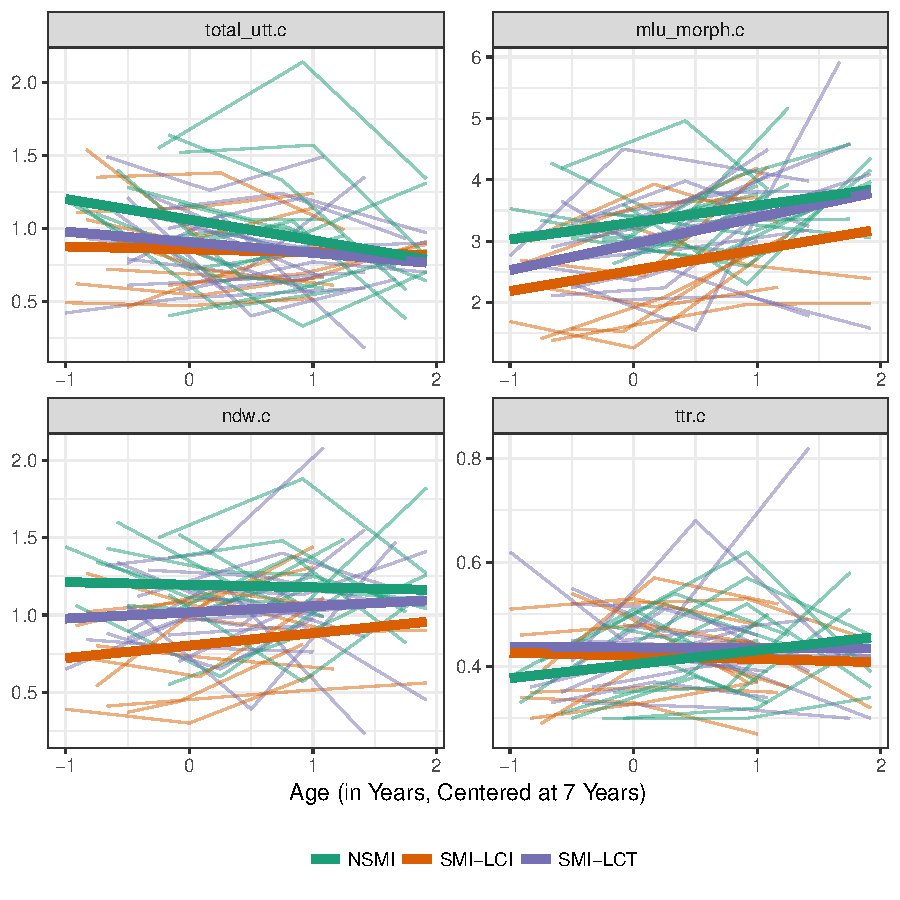
\includegraphics[width=1\linewidth]{fitted_plots_for_speech_analysis_speech_for_handout.pdf}
\captionof{figure}{Each subject, color coded by group, for each outcome.}
\label{fig:cp}
\end{center}\vspace{0cm}
\hspace{.5cm}Clinicians categorize these children into 3 categories based off of speech ability. One of our goals was to see if the data-driven methods regarding analysis of speech patterns collected on 35 children in the cohort suggested existence of these clinical categories.  Figure \ref{fig:cp} shows the subject level data for 4 speech variables of interest with the fitted values from a multivariate longitudinal model overlaid for each group.


\subsubsection*{Power Analysis for Longitudinal Data Using Decomposition}
Power analysis and sample size calculations are a crucial component of any study design. However, many study designs lead to either complicated formulas or do not have closed form solutions. We propose a method for calculating power in the situation of clustered or longitudinal data that leads to a solution that is both simple to calculate and gives valuable insight to how study design parameters affect power.
\begin{center}\vspace{0cm}
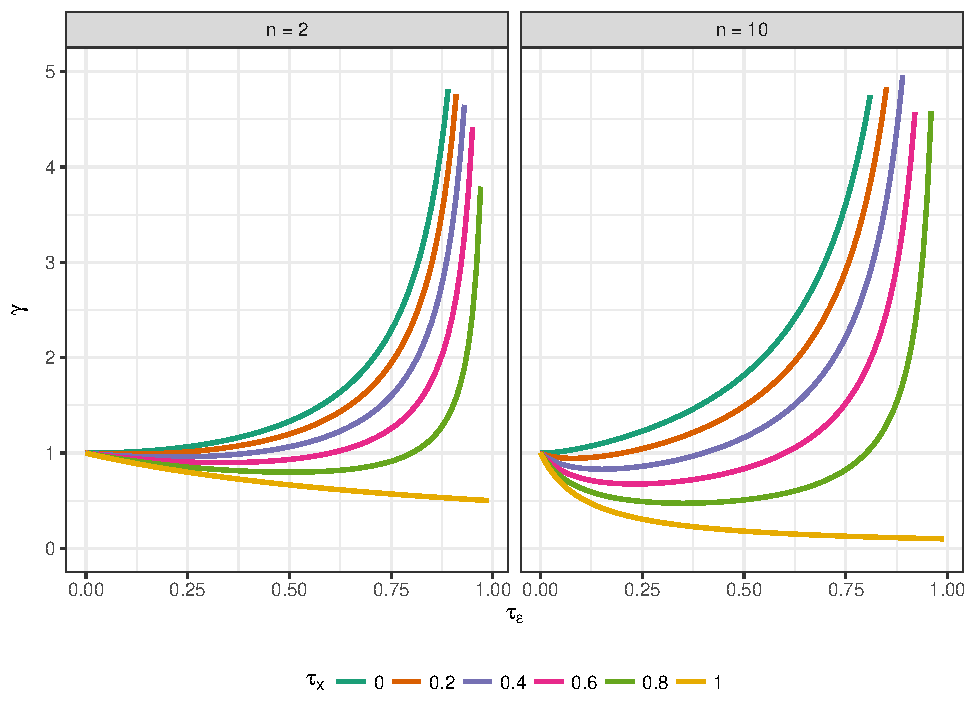
\includegraphics[width=1\linewidth]{gamma_analysis.pdf}
\captionof{figure}{Parameter $\gamma$ for different study design parameters, $\tau_\epsilon, \tau_x$, and $n$.}
\label{fig:gamma}
\end{center}\vspace{0cm}
\hspace{.5cm}We consider the situation where covariates are randomly observed. Our model of interest is,
\begin{equation} \label{eq:model}
Y_{i,j}=\beta_0+ \beta X_{i,j}+ \epsilon_{i,j},
\end{equation}
where $i=1,\ldots, m$ and $j=1,\ldots,n$ denote the study participant and observation within participant, respectively. We expect measurements within subject to be positively correlated. Therefore, corr$(X_{i,j},X_{i,j'}) = \tau_X >0$ and corr$(\epsilon_{i,j},\epsilon_{i,j'}) = \tau_\epsilon>0$. Finally, $\mbox{Var}(X_{i,j}) = \mbox{Var}(\epsilon_{i,j}) =1$, Using an approach which decomposes the covariates, we are able to come to a power formula with two parts; one part is the correlation between $X_{i,j}$ and $Y_{i,j}$ without accounting for the correlation within subjects, and another part, $\gamma$, is a function of study design parameters. This equation is shown below, 
\begin{equation} \label{eq:rhoeff}
\rho^2_{\mbox{eff}} =\frac{\rho^2\gamma}{\rho^2\gamma+(1-\rho^2)}.
\end{equation}
\noindent Figure \ref{fig:gamma} shows how $\gamma$ varies as different study design parameters change. There are interesting special cases of this result. For example, when $\tau_X = \tau_\epsilon$, this is equivalent to an independent random sample, and when $\tau_X= 1$ we recover the classical result for longitudinal studies comparing treatment to control group.

\end{multicols}
\end{document}